\documentclass{article}
\usepackage[utf8]{inputenc}
\usepackage{graphicx}
\usepackage{booktabs}
\usepackage{amsmath}
\usepackage{biblatex}
\addbibresource{referencias.bib}

% Comandos automáticos para a capa
\newcommand{\instituicao}{Centro Federal de Educação Tecnológica de Minas Gerais}
\newcommand{\programa}{Pós-Graduação em Modelagem Matemática Computacional}
\newcommand{\curso}{Algoritmos e Estruturas de Dados}
\newcommand{\autor}{Leonardo Vieira Guimarães}
\newcommand{\titulo}{Relatório - Trabalho Prático: Caixeiro Viajante (TSP)}
\newcommand{\cidade}{Belo Horizonte}
\newcommand{\dataentrega}{Julho de 2025}

\begin{document}

% Capa automática padrão ABNT com tamanhos e espaçamentos aprimorados
\begin{titlepage}
    \begin{center}
        % Instituição, programa e curso
        {\fontsize{12}{16}\selectfont \instituicao}\\[0.7cm]
        {\fontsize{12}{16}\selectfont \programa}\\[0.7cm]
        {\fontsize{12}{16}\selectfont \curso}\\[0.7cm]
        % Autor
        {\fontsize{12}{16}\selectfont \textbf{\autor}}\\[6cm]
        % Título
        {\fontsize{18}{20}\selectfont \MakeUppercase{\textbf{\titulo}}}\\[7cm]
        % Cidade e data (juntos na mesma linha)
        {\fontsize{14}{16}\selectfont \cidade\ --- \dataentrega}
    \end{center}
\end{titlepage}
\thispagestyle{empty}
\newpage
\renewcommand{\contentsname}{Sumário}
\tableofcontents
\newpage

\section{Introdução}
Este relatório apresenta a análise experimental dos algoritmos de força bruta e heurística para o problema do Caixeiro Viajante (TSP), conforme solicitado no trabalho prático da disciplina. O objetivo é comparar o desempenho e a qualidade das soluções obtidas por cada abordagem.

\subsection*{Objetivo do Trabalho}
Implementar algoritmo de força bruta e uma heurística para o problema do Caixeiro Viajante (TSP).

O trabalho é composto de duas partes:
\begin{itemize}
    \item Aplicação do algoritmo de força-bruta em instâncias do problema do caixeiro viajante.
    \item Aplicação de uma heurística em três instâncias do mesmo problema.
\end{itemize}

O problema do Caixeiro Viajante consiste em, dado um conjunto de cidades onde existe um caminho entre cada par de cidades com uma distância positiva, encontrar um caminho que, a partir de uma cidade, visita todas as cidades e retorna à cidade inicial percorrendo a menor distância possível.


\section{Metodologia}

Os experimentos foram realizados utilizando Python, sendo realizados em duas etapas, parte 1 com implementação de força brue e parte 2 com implementação de heurística.

\subsection{Parte 1: Força Bruta}

A abordagem de força bruta para o TSP consiste em gerar todas as rotas possíveis que visitam cada cidade exatamente uma vez e retornam ao ponto de origem, calculando o custo total de cada percurso e selecionando o de menor valor~\cite{lawler1985tsp}. Devido à sua complexidade fatorial ($O(n!)$), essa estratégia é restrita a instâncias pequenas, normalmente até 12 cidades. As etapas desta parte do trabalho foram:

\begin{enumerate}
    \item \textbf{Implementação do algoritmo:} Desenvolvimento do método de força bruta para identificar a rota de menor custo dentre todas as possíveis.
    \item \textbf{Geração das instâncias:} Criação automática de instâncias aleatórias, variando de 2 até o limite viável de cidades, com pesos aleatórios entre as cidades.
    \item \textbf{Execução e análise:} Aplicação do algoritmo a cada instância gerada, com registro do tempo de execução para análise do crescimento exponencial do custo computacional.
    \item \textbf{Representação do grafo:} Utilização da matriz de adjacência, em que o elemento $(i, j)$ indica a distância entre as cidades $i$ e $j$, por ser mais adequada para grafos densos como o TSP e facilitar o acesso aos dados.
\end{enumerate}


\subsection{Parte 2: Heurística}

A heurística do vizinho mais próximo foi escolhida para abordar instâncias de maior porte do TSP. Essa heurística constrói uma solução de forma gulosa: a cada passo, parte da cidade atual e visita a cidade mais próxima ainda não visitada, até completar o ciclo~\cite{ufpr_tsp}. 

A heurística do vizinho mais próximo é uma abordagem construtiva e gulosa, bastante utilizada para instâncias grandes do TSP por ser simples e rápida. O algoritmo parte de uma cidade inicial e, a cada etapa, visita a cidade não visitada mais próxima, repetindo o processo até percorrer todas as cidades e retornar ao ponto de partida~\cite{miy2008heuristicas}. Embora não garanta a solução ótima, é eficiente e serve como referência ou ponto de partida para métodos mais sofisticados.

As etapas desta parte do trabalho foram:

\begin{enumerate}
    \item \textbf{Implementação da heurística:} Desenvolvimento do algoritmo do vizinho mais próximo para encontrar uma solução aproximada para o TSP.
    \item \textbf{Aplicação nas instâncias reais:} A heurística foi aplicada às três instâncias fornecidas no Moodle, cada uma com características específicas:
        \begin{itemize}
            \item \textbf{si535.tsp}: Instância com 535 cidades, fornecida apenas com a diagonal superior da matriz de adjacência. Foi necessário reconstruir a matriz completa para aplicação do algoritmo.
            \item \textbf{pa561.tsp}: Instância com 561 cidades, fornecida apenas com a diagonal inferior da matriz de adjacência. Também foi implementada uma função para reconstruir a matriz completa.
            \item \textbf{si1032.tsp}: Instância com 1032 cidades, igualmente fornecida apenas com a diagonal superior, exigindo reconstrução da matriz de adjacência.
        \end{itemize}
    \item \textbf{Verificação dos resultados:} Após a execução da heurística, foi registrada a distância total encontrada para cada instância, permitindo a análise da qualidade das soluções obtidas.
\end{enumerate}

\section{Resultados e Discussão}

Foram realizados experimentos com o algoritmo de força bruta e a heurística do vizinho mais próximo, conforme descrito nas seções anteriores. A seguir, são apresentados os resultados obtidos, da parte 1 para força bruta e parte 2 para a heurística do vizinho. 

\subsection{Parte 1: Resultados Força Bruta}


Nesta etapa, foi implementado o algoritmo de força bruta para resolver o TSP. Para ilustrar seu funcionamento, foram realizadas execuções em instâncias variando de 2 até 13 cidades. A matriz apresentada na Equação~\ref{matriz_5_cidades_forca_bruta} exemplifica o caso para 5 cidades, onde cada elemento $(i, j)$ indica a distância entre as cidades $i$ e $j$. A Figura~\ref{fig:grafo_5_cidades_forca_bruta} mostra o grafo correspondente a essa matriz de adjacência.

\begin{equation}
\label{matriz_5_cidades_forca_bruta}
\begin{bmatrix}
0 & 8 & 6 & 77 & 83 \\
8 & 0 & 96 & 56 & 65 \\
6 & 96 & 0 & 10 & 17 \\
77 & 56 & 10 & 0 & 29 \\
83 & 65 & 17 & 29 & 0
\end{bmatrix}
\end{equation}

begin{figure}[h!]
\begin{figure}[h!]
    \centering
    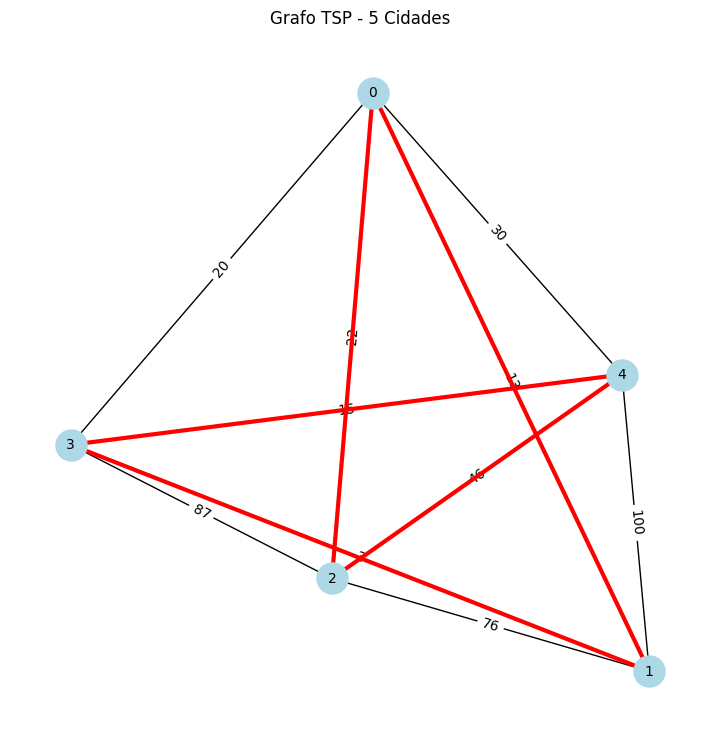
\includegraphics[width=0.6\textwidth]{../graficos/grafo_5_cidades.png}
    \caption{Grafo correspondente à matriz de adjacência para 5 cidades.}
    \label{fig:grafo_5_cidades_forca_bruta}
\end{figure}

Para essa instância passando por todas cidades com a menor distância a melhor rota encontrada foi [0, 1, 3, 4, 2, 0], com distância total de 99, para execução desse algoritmo para 5 cidades gastou um tempo de 0.0002 segundos.

O algoritmo foi aplicado em instâncias variando de 2 até 13 cidades, registrando o tempo de execução e a distância ótima obtida em cada caso. O comportamento do tempo de execução em função do número de cidades pode ser visualizado na Figura~\ref{fig:tempo_forca_bruta}.

\begin{figure}[h!]
    \centering
    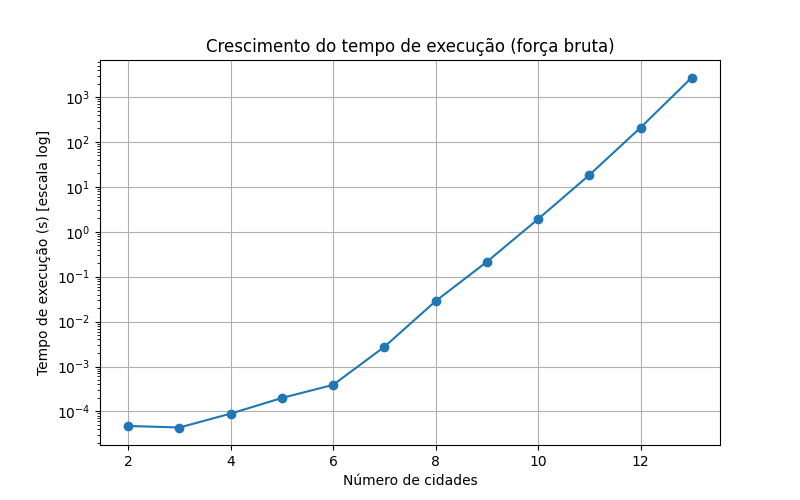
\includegraphics[width=0.8\textwidth]{../graficos/grafico_tempo_forca_bruta.png}
    \caption{Tempo de execução do algoritmo de força bruta em escala logarítmica.}
    \label{fig:tempo_forca_bruta}
\end{figure}

\noindent Observa-se que o tempo cresce rapidamente, tornando o método impraticável para instâncias maiores que 12 cidades.

\subsection{Parte 2: Resultados da Heurística}

Nesta etapa, foi implementada a heurística do vizinho mais próximo para encontrar uma solução aproximada para o TSP. O mesmo procedimento de teste foi realizado para instâncias variando de 2 até 13 cidades. Para ilustrar o funcionamento do método, aplicou-se a heurística em uma instância com 5 cidades, utilizando a matriz de adjacência apresentada anteriormente. O resultado obtido foi:

\begin{equation}
\label{matriz_5_cidades_heuristica}
\begin{bmatrix}
0 & 51 & 96 & 54 & 9 \\
51 & 0 & 73 & 13 & 56 \\
96 & 73 & 0 & 77 & 54 \\
54 & 13 & 77 & 0 & 13 \\
9 & 56 & 54 & 13 & 0
\end{bmatrix}
\end{equation}


\begin{figure}[h!]
    \centering
    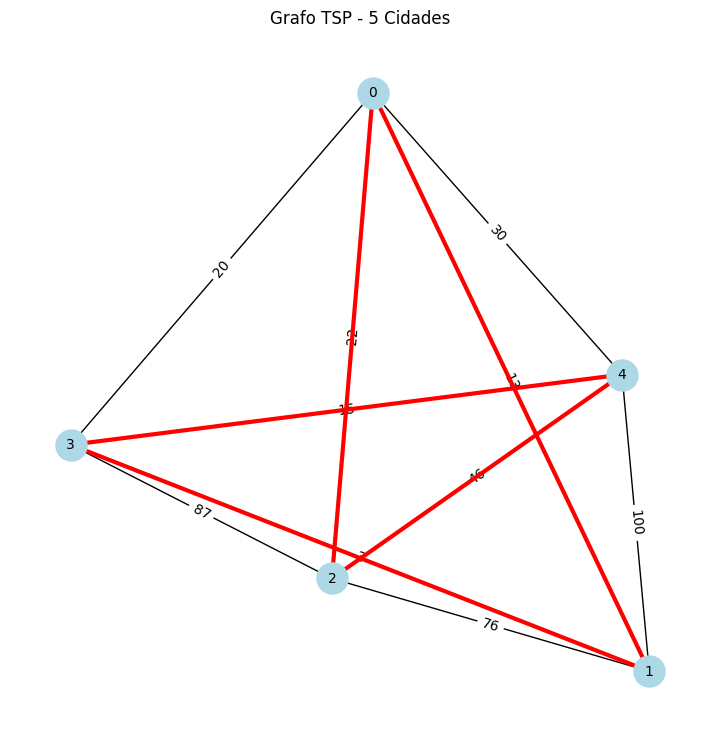
\includegraphics[width=0.6\textwidth]{../graficos/grafo_5_cidades.png}
    \caption{Grafo correspondente à matriz de adjacência para 5 cidades.}
    \label{fig:grafo_heuristica_5_cidades}
\end{figure}

Para essa instância passando por todas cidades com a menor distância a melhor rota encontrada foi [0, 4, 3, 1, 2, 0], com distância total de 204, para execução desse algoritmo para 5 cidades gastou um tempo de 0.0000 segundos.

O algoritmo foi aplicado em instâncias variando de 2 até 14 cidades, registrando o tempo de execução e a distância encontrada pela heurística em cada caso. O comportamento do tempo de execução em função do número de cidades pode ser visualizado na Figura~\ref{fig:tempo_heuristica}.

\begin{figure}[h!]
    \centering
    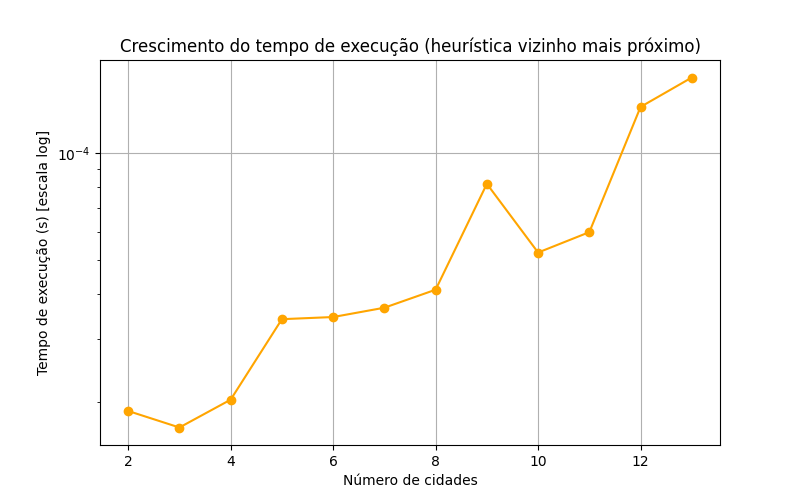
\includegraphics[width=0.8\textwidth]{../graficos/grafico_tempo_heuristica.png}
    \caption{Tempo de execução da heurística do vizinho mais próximo em escala logarítmica.}
    \label{fig:tempo_heuristica}
\end{figure}

\noindent Observa-se que o tempo de execução cresce de forma linear, indicando a eficiência da heurística mesmo para instâncias maiores.

Em seguida, a heurística foi aplicada nas três instâncias reais fornecidas, cujas matrizes de adjacência estão disponíveis nos formatos diagonal superior ou inferior. Para cada arquivo, foi utilizada uma função de leitura específica para reconstruir a matriz completa e garantir a correta execução do algoritmo.

A Tabela~\ref{tab:heuristica} apresenta as distâncias totais encontradas pela heurística do vizinho mais próximo para cada instância fornecida:

\begin{table}[h!]
    \centering
    \begin{tabular}{lcc}
        \toprule
        Instância & Número de cidades & Distância encontrada \\
        \midrule
        si535.tsp  & 535  & 50144 \\
        pa561.tsp  & 561  & 3422 \\
        si1032.tsp & 1032 & 94571 \\
        \bottomrule
    \end{tabular}
    \caption{Distâncias encontradas pela heurística do vizinho mais próximo}
    \label{tab:heuristica}
\end{table}

\section{Considerações Finais}

Os experimentos realizados permitiram comparar o desempenho do algoritmo de força bruta e da heurística do vizinho mais próximo para o problema do Caixeiro Viajante (TSP). O método de força bruta mostrou-se adequado apenas para instâncias pequenas, devido ao crescimento exponencial do tempo de execução, mas foi fundamental para validar a implementação e servir de referência para a avaliação das heurísticas. Por outro lado, a heurística do vizinho mais próximo demonstrou ser eficiente e capaz de fornecer soluções aproximadas em tempo viável mesmo para instâncias com centenas de cidades, embora não garanta a obtenção da solução ótima.

A comparação entre força bruta e heurística evidenciou que o método exato é viável apenas para poucos vértices, enquanto a heurística do vizinho mais próximo oferece soluções rápidas e razoáveis para instâncias grandes. O código-fonte está disponível publicamente para consulta e reprodução dos experimentos~\cite{guimaraes2025github}.

% Bloco de referências
\printbibliography
\end{document}
